\chapter{Thème: Somme de deux dés}
{ }\hfill\textbf{Niveau:} Moyen\\ \\
Lorsqu'on lance deux dés et qu'on fait le total des points de chacun des dés, on obtient un entier compris entre 2 et 12. Ici, nous allons voir dans cette activité la répartition des différents tirages et la représenter sous forme d'un petit graphique.
\section{Simuler le lancer d'un dé.}
\noindent Pour simuler le lancer d'un dé, nous allons utiliser la primitive \texttt{hasard}. Voici comment procéder.\\ \\
\texttt{hasard 6} $\longrightarrow$ renvoie un entier pris au hasard parmi 0, 1, 2, 3, 4, 5.\\
Par conséquent, \texttt{(hasard 6)+1 } renvoie un entier pris au hasard parmi 1, 2, 3, 4, 5, 6. Noter bien les parenthèses, sinon l'interpréteur Logo comprendrait \texttt{hasard 7}. Pour éviter les parenthèses, on peut taper également \texttt{1+hasard 6}.\\ \\
On définit ainsi la procédure \texttt{lancer} qui simule le lancer d'un dé.
\begin{verbatim}
 pour lancer
   retourne 1+hasard 6
 fin
\end{verbatim}
 \section{Le programme}
  Nous allons utiliser le mode multi-tortues. Pour disposer ainsi de plusieurs tortues sur l'écran, on utilise la primitive \texttt{fixetortue} suivi du numéro de la tortue que l'on veut sélectionner.\\
  Un bon schéma valant mieux que mille explications....
\begin{center}
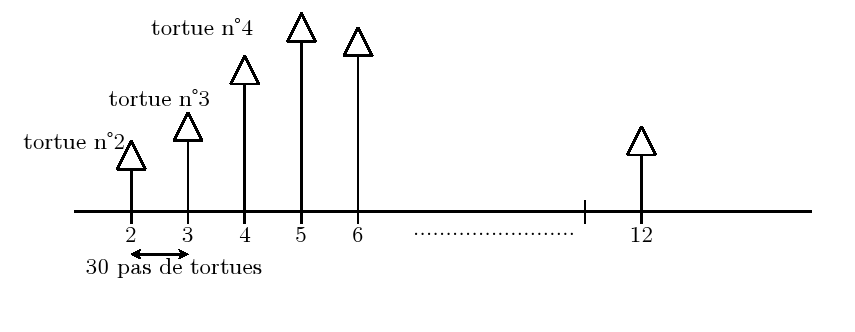
\includegraphics[scale=0.45]{images/somme-des-schema.png}
\end{center}
\vspace{0.5cm}
Sur le principe, chaque tortue numérotée de 2 à 12 avancera d'un pas de tortue, lorsque le tirage de la somme des deux dés sera identique à son numéro. Par exemple, si les dés ont pour somme 8, la tortue numéro 8 avancera d'un pas. Toutes les tortues sont espacées de 30 pas de tortues horizontalement.\\ \\
On placera les tortues à l'aide des coordonnées.
\begin{itemize}
 \item  La tortue n\degre2 sera placée en $(-150;0)$
 \item  La tortue n\degre3 sera placée en $(-120;0)$
 \item  La tortue n\degre4 sera placée en $(-90;0)$
 \item  La tortue n\degre5 sera placée en $(-60;0)$\\
\begin{minipage}{8 cm}
\begin{center}
 $\vdots$
\end{center}
\end{minipage}
\end{itemize}
\begin{verbatim}
 fixetortue 2 fpos [-150 0]
 fixetortue 3 fpos [-120 0]
 fixetortue 4 fpos [-90 0]
 fixetortue 5 fpos [-60 0]
 fixetortue 6 fpos [-30 0]
.....
\end{verbatim}
Plutôt que de taper 11 fois quasiment la même ligne de commande, on peut automatiser cela en utilisant la primitive \texttt{repetepour}. A l'aide de cette primitive, on peut affecter à une variable une succession de valeurs prises dans un intervalle à espaces réguliers. Ici, on veut que la variable \texttt{:i} prenne successivement les valeurs 2, 3, 4, ... , 12. On tapera:\\
\texttt{repetepour [i 2 12] [ liste des instructions à exécuter ]}\\ \\
Pour placer les tortues, on crée donc la procédure \texttt{initialise}
\begin{verbatim}
pour initialise
  ve ct
  repetepour [i 2 12] [ 
      # On place la tortue
      fixetortue :i fpos liste -150+(:i-2)*30 0
      # On écrit le numéro de la tortue juste en dessous 
      lc re 15 etiquette :i av 15 bc 
  ]
fin
\end{verbatim}

Bien comprendre la formule \texttt{-150+(:i-2)*30}. On part de -150, puis à chaque nouvelle tortue on rajoute 30. (Tester avec les différentes valeurs de \texttt{:i} si vous n'êtes pas convaincu)\\ \\
Au final on obtient le programme suivant:
\begin{verbatim}
pour lancer
 retourne 1+hasard 6
fin

pour initialise
  ve ct
  repetepour [i 2 12] [ 
      # On place la tortue
      fixetortue :i fpos liste -150+(:i-2)*30 0
      # On écrit le numéro de la tortue juste en dessous 
      lc re 15 etiquette :i av 15 bc 
  ]
fin

pour demarrer
initialise
# On effectue 1000 tentatives
repete 1000 [
  donne "somme lancer+lancer
  fixetortue :somme av 1
]
# On affiche les fréquences de tirage
repetepour [i 2 12] [
  fixetortue :i
  # L'ordonnée de la tortue représente le nombre de tirages
  soit "effectif dernier pos 
  lc av 10 tg 90 av 10 td 90 bc etiquette :effectif/1000*100
]
fin
\end{verbatim}
\pagebreak
Voici une généralisation de ce programme. Ici, on demandera à l'utilisateur le nombre de dés souhaités ainsi que le nombre de lancers à effectuer.
\begin{verbatim}
pour lancer
soit "somme 0
repete :des [
   soit "somme :somme+1 +hasard 6
 ]
retourne :somme
fin

pour initialise
  ve ct fixemaxtortues :max+1
  repetepour ph liste "i :min :max [ 
      # On place la tortue
      fixetortue :i fpos liste (:min-:max)/2*30+(:i-:min)*30 0
      # On écrit le numéro de la tortue juste en dessous 
      lc re 15 etiquette :i av 15 bc 
  ]
fin

pour demarrer
lis [Nombre de dés:] "des
si non nombre? :des [ec [Le nombre rentré n'est pas valide!] stop]
donne "min :des
donne "max 6*:des
lis [Nombre de lancers à effectuer] "tirages
si non nombre? :tirages [ec [Le nombre rentré n'est pas valide!] stop]
initialise
# On effectue 1000 tentatives
repete :tirages [
  fixetortue lancer av 1
]
# On affiche les fréquences de tirage
repetepour ph liste "i :min :max [
  fixetortue :i
  # L'ordonnée de la tortue représente le nombre de tirages
  soit "effectif dernier pos 
  # On arrondit à 0,1
  lc av 10 tg 90 av 10 td 90 bc etiquette (arrondi :effectif/:tirages*1000)/10
]
fin

\end{verbatim}